\documentclass{amsart}
\usepackage{}
\usepackage{tikz}
\usetikzlibrary{arrows.meta}
\begin{document}
\title{Vehicle Priority Queues on Two-Lane Roads}
\author{David Prentiss}
\date{\today}
\maketitle
\section{Motivation}

\cite{Prentiss2020}
\cite{Levin2019a}
\cite{LeVine2016a}
\cite{Dresner2004}

\section{Queueing model}
Consider a two-way, two-lane road segment connecting two at-grade, controlled
intersections. Suppose that in one direction, vehicles arrive at the upstream
end of their respective lane according to a Poisson process with mean arrival
rate $\lambda$. We will, for the moment, ignore the other lane.

Suppose also, that arriving vehicles are in one of two classes, $A$ or $B$.
Furthermore vehicles in each class arrive in equal proportion such that their
respective mean arrival rates are $\lambda_A=\lambda_B=\lambda/2$. We leave the
practical difference between the two classes deliberately abstract. However, it
may be useful to think of the two classes as being different intended turning
motions. For now, the only practical difference is that the downstream
intersection controls will admit only one class or the other in a single phase.
Equivalently, we could say that, during a single phase the intersection admits
all and only the vehicles of the same class that happen to be adjacent to each
other at the head of the queue. For example, if the sequence of vehicles
starting from the head of the queue had classes $\{A,B,B,A,A,A,B,B\}$, then the
intersection would, in sequential phases, admit one vehicle of type $A$, then
two vehicles of type $B$, then three vehicles of type $A$, and so on.

For the purposes of analysis, we make the following, additional simplifying
assumptions regarding vehicle dynamics. First, time and space are discretized
such that each vehicle takes the space of one cell and can move, at most, one
cell per time step. The time then, for $n$ vehicles to enter the intersection is
$T_n=n$ steps, where $n$ is a random variable representing the number of
vehicles admitted through the intersection during a given phase. Second,
vehicles that enter the intersection are considered to have left the system. And
third, the time until the next phase is $T_n+T_p$, where $T_n = t(n)$ and $T_p$
is a random variable representing the time necessary for the intersection to
complete some other, mutually exclusive activities such as another phase for
vehicles in other, un-modeled legs. For now, we will say of $T_p$ only that it
is i.i.d.\ as $T_n$.

\subsection{Typical two-lane road with batch service}
We will take expected rate of departure, $\mu$ to be the expected value of
\begin{equation*}
  \frac{n}{T_n+T_p}.
\end{equation*}
Since $T_n=n$ steps/vehicle, then $\text{E}[n]=\text{E}[T_n]$ vehicles.
That is, the expected number of steps it takes the next group of vehicles to
enter the intersection is equal to the expected number of vehicles in that
group. So we have
\begin{equation}
  \mu = \text{E}\left[\frac{n}{T_n+T_p}\right]
  =\text{E}\left[\frac{n}{n+n}\right] = \frac{1}{2}\text{ (vehicles/step)}.
\end{equation}

\subsection{Moving the stop bar}
Now suppose that we moved the stop bar upstream of the intersection some number
of cells $k$, where $0\leq k<L$.
That is, rather than vehicles forming a queue directly adjacent to the
intersection, the head of the queue now waits $k$ cells away.
Then $\text{E}[T_n]=\text{E}[T_p]=\text{E}[n]+k$ and
\begin{equation*}
  \mu = \text{E}\left[\frac{n}{T_n+T_p}\right]
  = \text{E}\left[\frac{n}{2(n+k)}\right]
  = \frac{1}{2}\text{E}\left[\frac{n}{n+k}\right]\text{ (vehicles/step)}.
\end{equation*}
Since the interarrival time distributions of vehicles in each class are i.i.d.\ and
$\lambda_A=\lambda_B$, the probability that any given arriving vehicle is in a
different class than the previous vehicle is $1/2$.
If we think of such an arrival as a ``success'' of a Bernoulli trial,
then $n\sim \text{Geo}(p=1/2)$ with support $m$ vehicles, where
$m\in\{1,2,3,\dots\}$, and mean $\text{E}[n]=1/p=2$.
So then,
\begin{equation}
  \mu=\frac{1}{2+k}\text{ (vehicles/step)}.
\end{equation}

\subsection{Priority queueing on two lanes}
We have so far ignored the adjacent, second lane. Suppose now that we appropriate that
lane exclusively for passing.
Furthermore, suppose that both lanes have length $L>1$ cells and that any
vehicles of the appropriate class may merge to the passing lane without conflict
and advance to and enter the intersection.
Finally we also assume that the arrival rate $\lambda$ is sufficiently large to
ensure that there are $L-k$ vehicles in the queue at the start of each phase.

Suppose, without loss of generality, that the current phase permits vehicles of
class $A$. Then the previous phase will have removed all vehicles of type $B$
from the queue and the remaining vehicles, of type $A$, will have moved to the
head of the queue, with the rest of the space being filled with newly queued
vehicles in equal proportions.
If the number of vehicles of type $B$ passed in the previous phase is $n_{p-1}$, then the number
of vehicles of type $A$ that moved to the head of the queue is
$n_p^*=L-k-n_{p-1}$,
and the number of vehicles, $n$, to be admitted this phase is $n_p^*$ plus the
proportion of $L -k-n_p^*$ newly arriving vehicles that are of type $A$.

For our assumed arrival rate means, it can be shown that for any initial
proportions of vehicles in the queue, $\text{E}[n]$ approaches
$\frac{2}{3}(L-k)$ in the limit of successive phases.
For now, it will suffice to consider a phase admitting type-$A$ vehicles that begins with
$\frac{2}{3}(L-k)$ type-$A$ vehicles in the queue.
After all type-$A$ vehicles have left the system, we are left with $\frac{1}{3}(L-k)$
vehicles of type $B$.
The newly arriving vehicles will, on average, have $\frac{1}{3}(L-k)$ vehicles of each type.
So the number of type-$B$ vehicles in the queue is $\frac{2}{3}(L-k)$ and
therefore in expectation, this phase is
equivalent to the last.

To find expected departure rate under this regime, we must also find the expected time it takes
for vehicles to leave the system during each phase.
Empirically, we find the mean to be $L-1$.
If $\text{E}[n] = \frac{2}{3}(L-k)$ and $\text{E}[T_n]=\text{E}[T_p]=L-1$, then
\begin{equation}
  \mu = \frac{\frac{2}{3}(L-k)}{2(L-1)}
  =\frac{L-k}{3(L-1)} \text{ (vehicles/step)}.
\end{equation}
\section{Model relaxation}
\begin{itemize}
\item More than two classes
\item Unequal arrival rates ($\lambda_A\neq\lambda_B$)
\item Lane not necessarily full ($\rho<1$)
\item Waiting phase different from active phase ($T_p$ not i.i.d.\ as  $T_n$)
\item Vehicles going the other direction
\end{itemize}
\section{To do}
\begin{itemize}
\item Find distribution for $n$ in priority case.
\item Find mean analytically and distribution for $T_n$ in priority case.
\end{itemize}

\bibliographystyle{amsplain}
\bibliography{bib/or647}

\end{document}

\section{Drafts}
\subsection{Equal length paths on a Manhattan grid}
\begin{figure}
  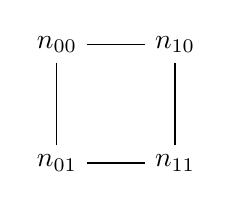
\begin{tikzpicture}[node distance={1.5cm}]
    \node (00) {$n_{00}$};
    \node (10) [right of=00] {$n_{10}$};
    \node (01) [below of=00] {$n_{01}$};
    \node (11) [right of=01] {$n_{11}$};

    \draw (00) edge (10);
    \draw (00) edge (01);
    \draw (10) edge (11);
    \draw (00) edge (10);
    \draw (01) edge (11);
  \end{tikzpicture}
\end{figure}
